
% \section{Gateway lunar}

% O \emph{Gateway Lunar}, conforme explica \cite{nasa_gateway}, está sendo desenvolvido pela NASA em colaboração com parceiros internacionais, como a ESA, JAXA e a CSA.
% Essa estação espacial servirá como centro de comunicações movido a energia solar, além de ser um laboratório científico e módulo habitacional de curto prazo.
% O \emph{Lunar Gateway} desempenhará um papel importante no programa Artemis, que facilitará a exploração lunar, e serve como ponto de partida para futuras missões tripuladas a Marte.

% Inicialmente, as primeiras estruturas serão o Elemento de Potência e Propulsão (PPE) e o Módulo de Habitação e Logística (HALO).
% O PPE fornecerá energia elétrica e a propulsão, enquanto que o HALO oferecerá espaço habitável para a tripulação e interfaces para integração de outras espaçonaves. Ambos os módulos estão programados para serem lançados juntos em 2027 a bordo de um foguete da \emph{SpaceX}.
% Além dos módulos descritos, o \emph{Lunar Gateway} contará a ESA para construir o módulo de reabastecimento e comunicações; a CSA contribuirá com um manipulador robótico de 8,5 metros, denominado \emph{Canadarm3} \cite{csa_canadarm3}.

% A órbita planejada para a estação espacial lunar é do tipo halo quase retilínea (NRHO), que permitirá acesso facilitado à superfície lunar.
% De acordo com \cite{esa_lunar_gateway_2019}, o Perilúnio será de 3.000 km e o Apolúnio será de 70.000 km.
% Essa órbita irá ajudar a melhorar comunicação com a Terra, reduzindo a falta de visada de forma que será uma plataforma estável para operações científicas diversas e de exploração.

% \begin{figure}[H]
%     \centering
%     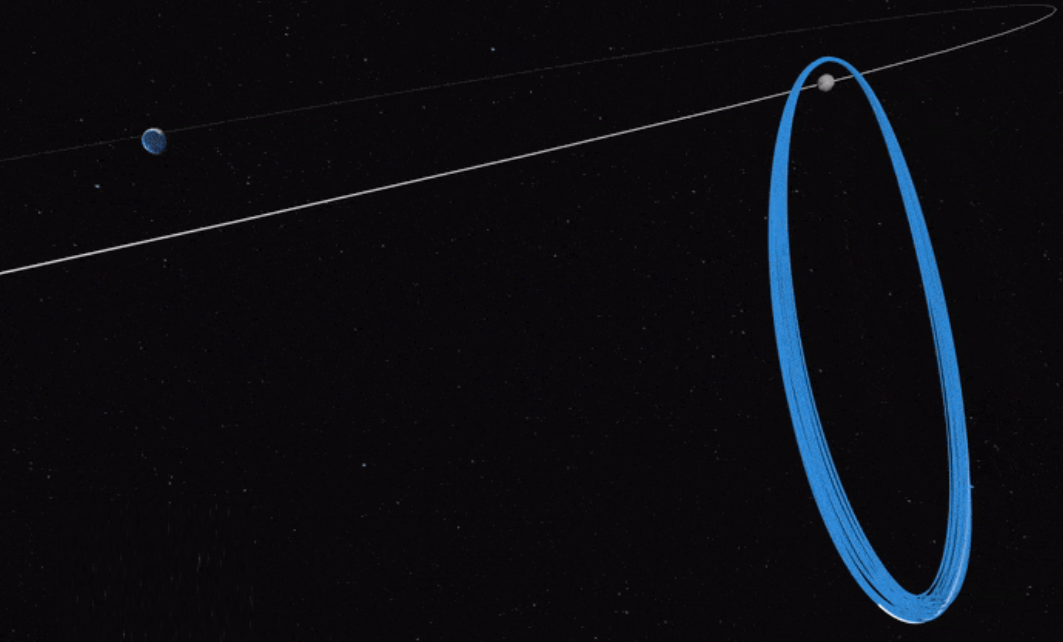
\includegraphics[width=1\linewidth]{1 Introducao/Imagens/Gateway lunar NRHO orbit.png}
%     \caption{Demonstração da órbita do Lunar Gateway. Fonte: ESA.}
%     \label{fig:orbitaGatewayNRHO}
% \end{figure}

% Para que toda a missão seja viável, é importante que os procedimentos de RVD/B entre os veículos espaciais e a estação sejam robustos e precisos, pois sem esse tipo de operação, a exploração futura não é possível.
% No contexto do \emph{Lunar Gateway}, essas manobras permitirão a chegada de tripulações, cargas, módulos adicionais e outros equipamentos, além de que irá viabilizar o retorno dos veículos espaciais à Terra.

\section{Gateway lunar}

O \emph{Gateway} lunar, desenvolvido pela \gls{nasa} em colaboração com parceiros internacionais \cite{nasaGateway}, é uma infraestrutura concebida para viabilizar operações cislunares com suporte logístico e científico.
Para este trabalho, o aspecto central do \emph{Gateway} é seu papel como nó orbital que depende de \gls{rvdb} para receber e integrar veículos de tripulação, cargueiros e módulos adicionais, além de suportar manobras de partida e retorno.

A arquitetura inicial inclui o Elemento de Potência e Propulsão (PPE) e o Módulo de Habitação e Logística (HALO), previstos para lançamento conjunto, fornecendo, respectivamente, energia/propulsão e interfaces para acoplamento e integração com outras espaçonaves \cite{nasaGateway}.
Adicionalmente, a contribuição canadense contempla um manipulador robótico (\emph{Canadarm3}), com implicações diretas para operações de captura, berthing e suporte a atividades de aproximação e integração de elementos \cite{csaCanadarm3}.

A órbita planejada do \emph{Gateway} é uma órbita halo quase retilínea (NRHO), escolhida para favorecer a acessibilidade à superfície lunar e manter condições operacionais adequadas para comunicações e logística \cite{esaLunarGateway2019}.
De acordo com \cite{esaLunarGateway2019}, o perilúnio é de 3.000~km e o apolúnio é de 70.000~km.

\begin{figure}[H]
    \centering
    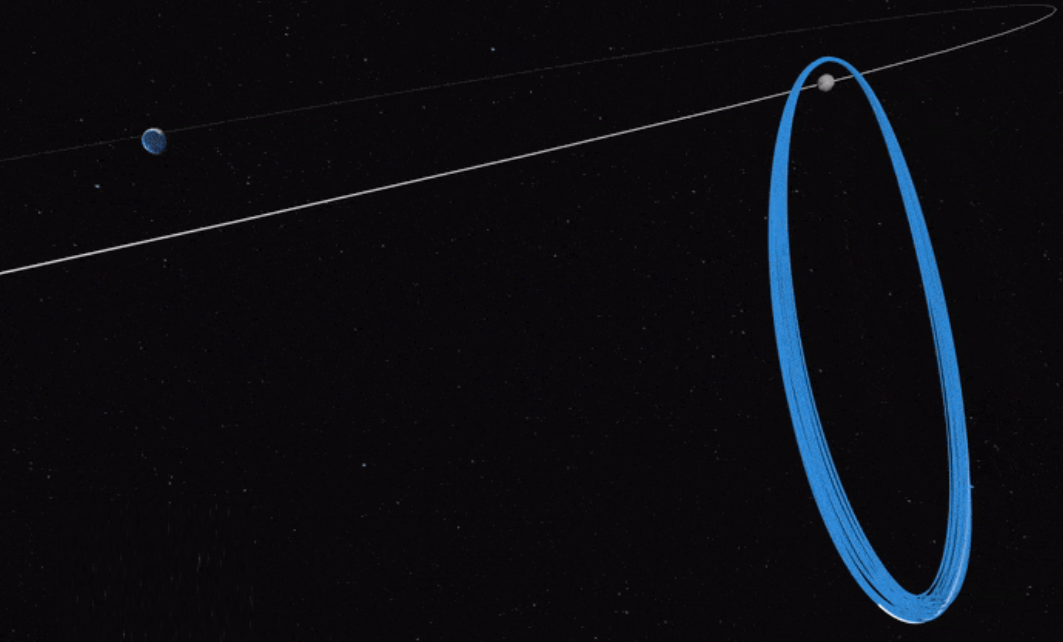
\includegraphics[width=1\linewidth]{1 Introducao/Imagens/Gateway lunar NRHO orbit.png}
    \caption{Demonstração da órbita do \emph{Gateway} lunar (NRHO). Fonte: ESA.}
    \label{fig:orbitaGatewayNRHO}
\end{figure}

A viabilidade operacional do \emph{Gateway} depende de procedimentos de \gls{rvdb} com precisão e confiabilidade compatíveis com o ambiente cislunar, em que restrições de comunicação e janelas de operação reduzem margens para intervenções imediatas.
Nesse cenário, \gls{rvdb} permite a chegada de tripulações e cargas, a integração progressiva de módulos e o suporte a sequências logísticas associadas às missões do programa \emph{Artemis} \cite{nasaGateway}.
